
\documentclass[10pt,a4paper]{article}

% Om het totaal aantal pagina's te tellen
\usepackage{lastpage}
\usepackage{graphicx}
\usepackage{listings}
% Om de marges aan te passen
\usepackage[left=2cm,right=2cm,top=2cm,bottom=2cm]{geometry}

% Voor headers en footers
\usepackage{fancyhdr}
\pagestyle{fancy}

\lhead{Giuseppe Callari and Xavier Go\'as Aguililla}
\rhead{\thepage /\pageref{LastPage}}

\lfoot{Assignment}
\cfoot{Computer Networks}
\rfoot{Network Simulation}

\renewcommand{\headrulewidth}{0.4pt}
\renewcommand{\footrulewidth}{0.4pt}

\begin{document}
\begin{titlepage}
\thispagestyle{empty}
\newcommand{\HRule}{\rule{\linewidth}{0.5mm}}
\center
\textsc{\LARGE KU Leuven}\\[1.5cm]
\vfill

% \HRule \\[0.4cm]
{ \Huge \bfseries Network simulation with NS/2}\\[0.4cm]
% \HRule \\[1.5cm]
\vfill

\begin{minipage}{0.4\textwidth}
\begin{flushleft} \large
\emph{Authors:}\\
Giuseppe \textsc{Callari} (r0301006)\\
Xavier \textsc{Go\'as Aguililla} (s0201506)
\end{flushleft}
\end{minipage}
~
\begin{minipage}{0.4\textwidth}
\begin{flushright} \large
\textsc{\large Computer networks [G0Q43A]}\\[0.5cm]
\emph{Professor:} \\
prof. dr. Daniel \textsc{Hughes}\\
\emph{Assistant:} \\
dr. Nelson \textsc{Matthys}\\
\end{flushright}
\end{minipage}\\[4cm]

{\large May 2nd, 2014}\\[3cm]
\vfill

\end{titlepage}


\tableofcontents
\newpage
\section{Exercise 1}
\subsection{Question 1 and 2}
In figure \ref{fig:lala} we can clearly see the difference between the
scenario with both an uploader and a downloader and that without an
uploader. In the scenario with an uploader, around the time the upload
starts (3.0s), the throughput for the downloader drops drastically. In
the scenario without an uploader, indicated in green, the throughput
of the connection remains roughly constant.

The download speed is limited by the link bandwidth. A maximum
throughput of about 475 packets per second is achieved, and we can
quickly calculate using the FTP packet size that this comes down to
about 475 packets/s $\cdot$ 1040 bytes/packet $\cdot$ 8 bits/byte
$\approx$ 4Mbps, which corresponds to the downstream link bandwidth of
the modem.

In figure \ref{fig:combined1} we see both the upload and download
throughput on the same graph; we can clearly see the aforementioned
drop in download speed at the moment the upload over CBR starts. The
speed is throttled to about the same as the upload (256Kbps). This is
due to the fact that both download packets destined for a node in the
LAN and download request packets departing the LAN have to pass
through the same node; both kinds of packets are generated at the same
rate, but due to the upload taking up all the upstream bandwidth, the
small request packets are transmitted at a much slower
rate. Accordingly, the download transfers are also started at a slower
rate, such that the download throughput is limited to that of the
upload. In a real scenario, this would not happen, since only one node
would be regulating the transfer; we do not have the bottleneck of
having to use two modem nodes.

\begin{figure}[p]
    \centering
    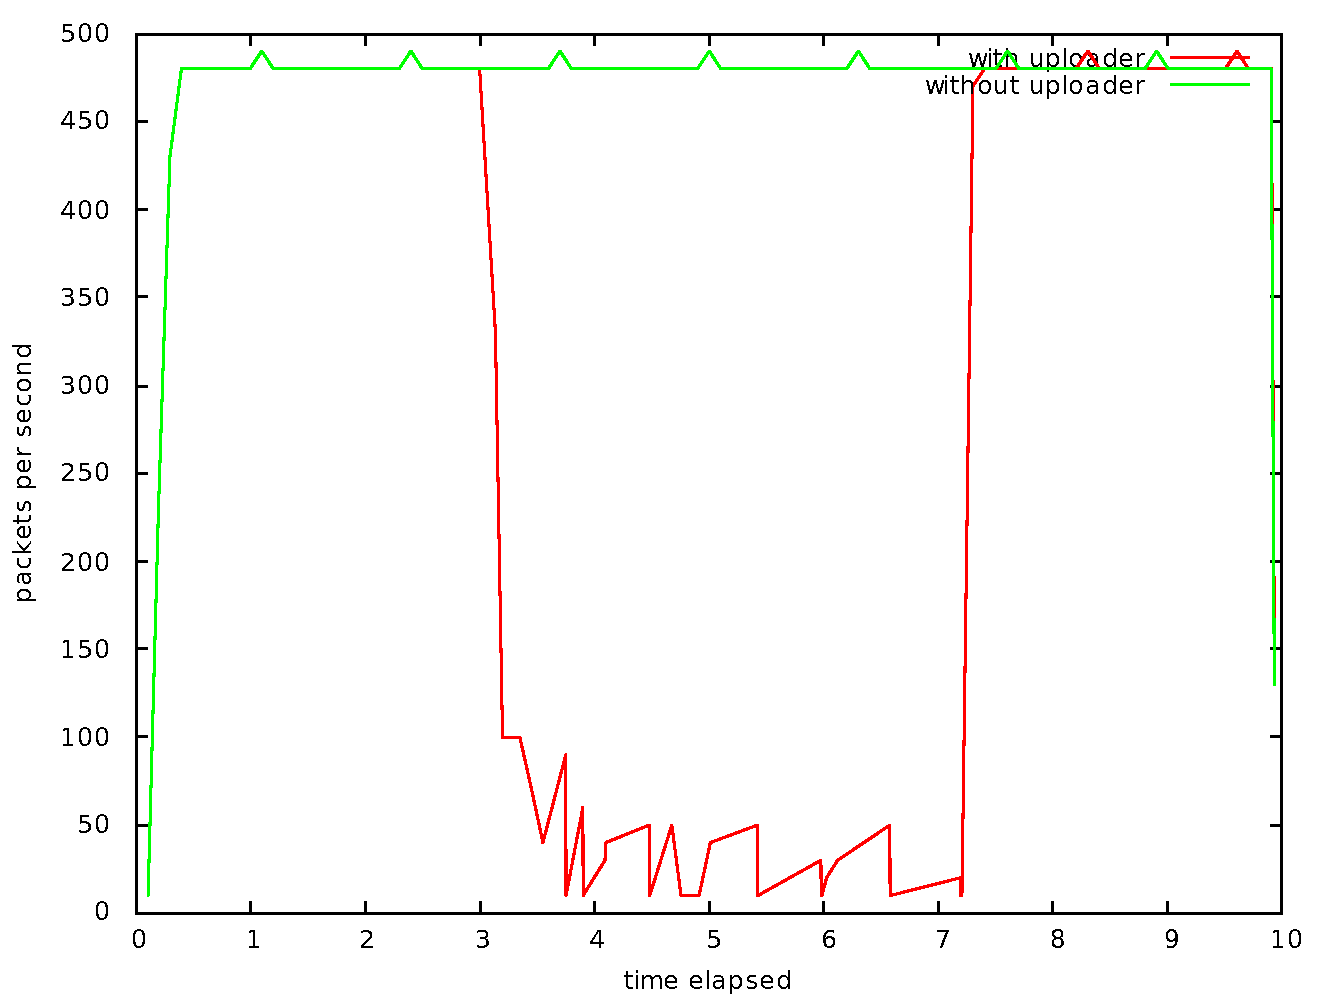
\includegraphics[width=\textwidth]{../part1/q1/plots/1.pdf}
    \caption{Download throughput compared}
    \label{fig:lala}
\end{figure}


\begin{figure}[p]
    \centering
    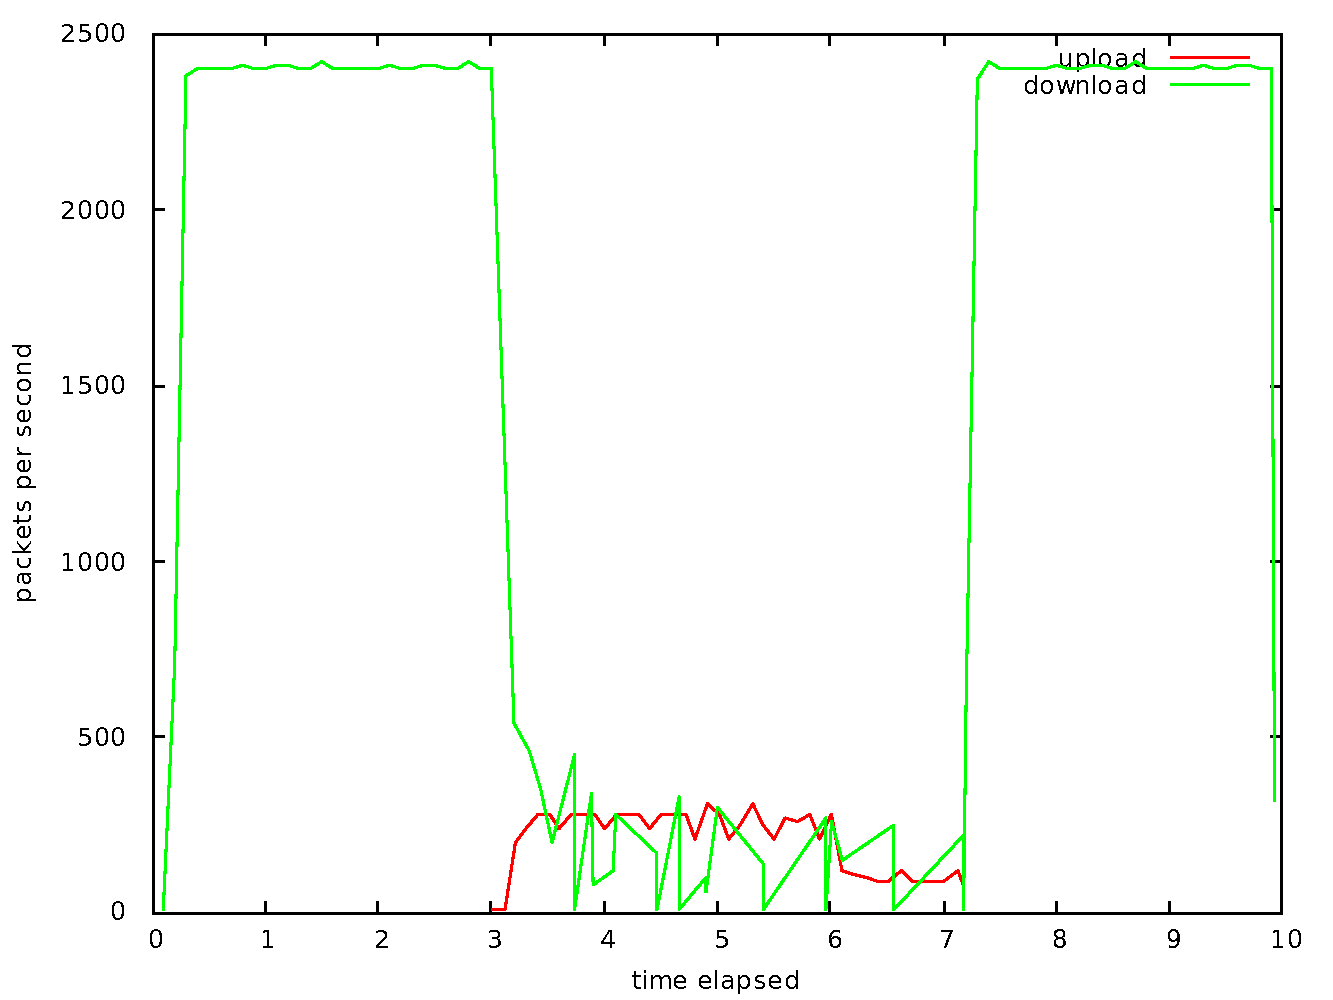
\includegraphics[width=\textwidth]{../part1/q2/plots/2.pdf}
    \caption{Upload and download throughput}
    \label{fig:combined1}
\end{figure}

\subsection{Question 3}

We expect performance for CBR to be excellent in this case, since a
certain amount of bandwidth is always guaranteed for the upload
connection. This does imply that the upload connection has a certain
privilege over the download connection; to ensure this, we could tell
the router to drop downstream packets rather than upstream
packets. This would result in increased packet loss for the download
connection, especially if we would run multiple upload connections at
the same time.

\subsection{Question 4}

We can see in figures \ref{fig:down_limited} and \ref{fig:up_limited} that
both the bridled and unbridled connection show similar patterns but
differ at the tail end of the speed drop from 3.0s on. At 6.0s the CBR
upload is stopped, but not all packets have been transferred yet due
to packet loss.

The connection layer ensures these lost packets still arrive at their
destination. To do this, the TCP connection persists while not all
packets have arrived at their destination. Looking at figure
\ref{fig:up_limited}, we see that the TCP upstream connection persists
longer in the situation with the limited bandwidth. The packets
transferred while the connection persists take up a certain amount of
bandwidth. Only around the 9.5 second mark are all the packets
transferred, and in figure \ref{fig:down_limited} we can see that the FTP
download is negatively affected by this transfer: the throughput is
very low until the 9.5 second mark.

\begin{figure}[p]
    \centering
    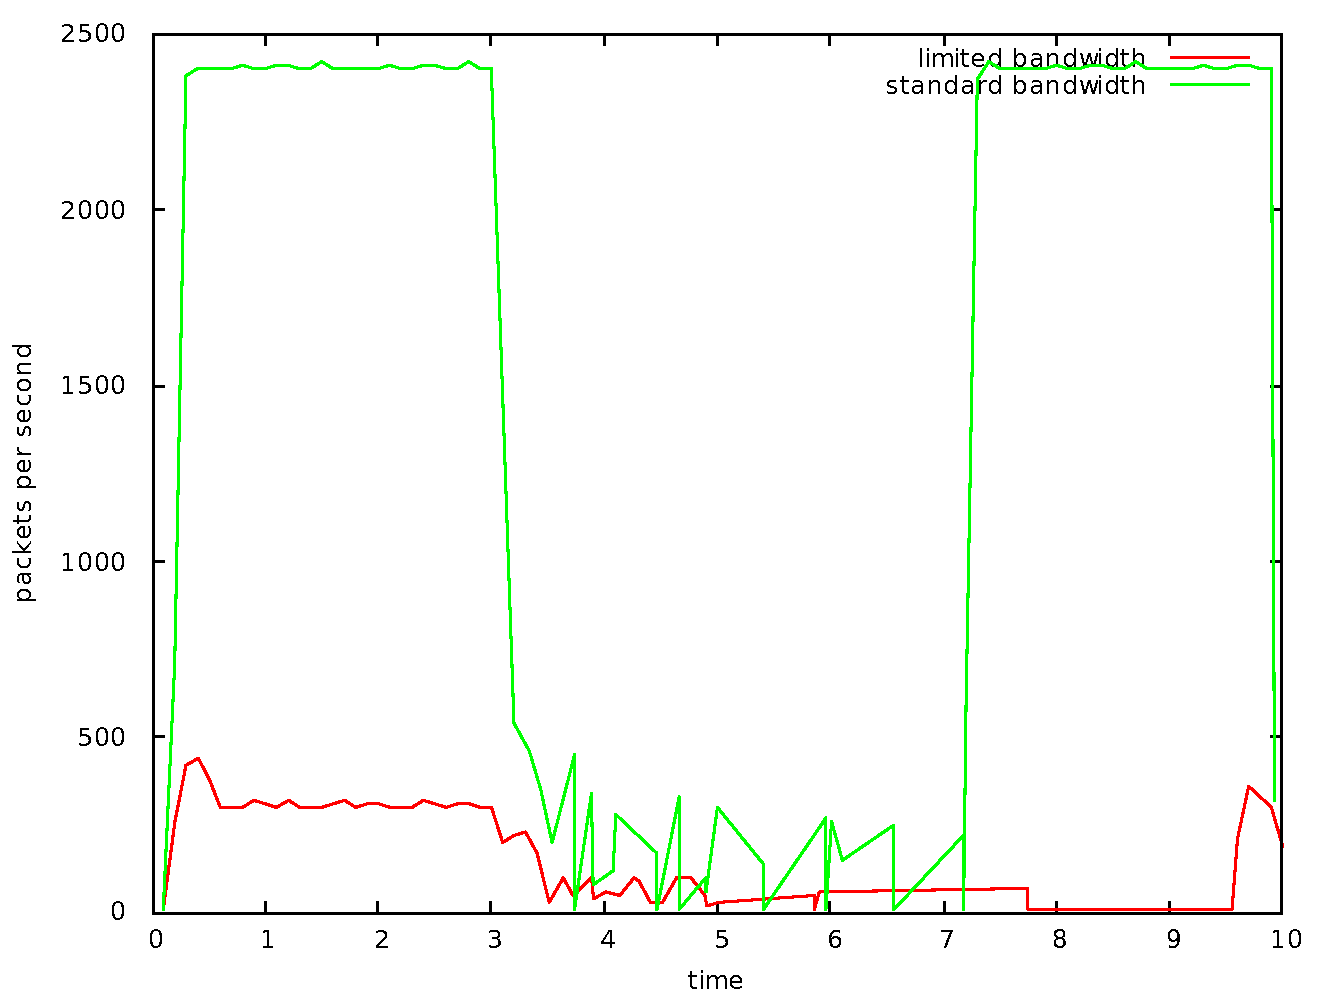
\includegraphics[width=\textwidth]{../part1/q4/plots/4-down.pdf}
    \caption{Download throughput}
    \label{fig:down_limited}
\end{figure}

\begin{figure}[p]
    \centering
    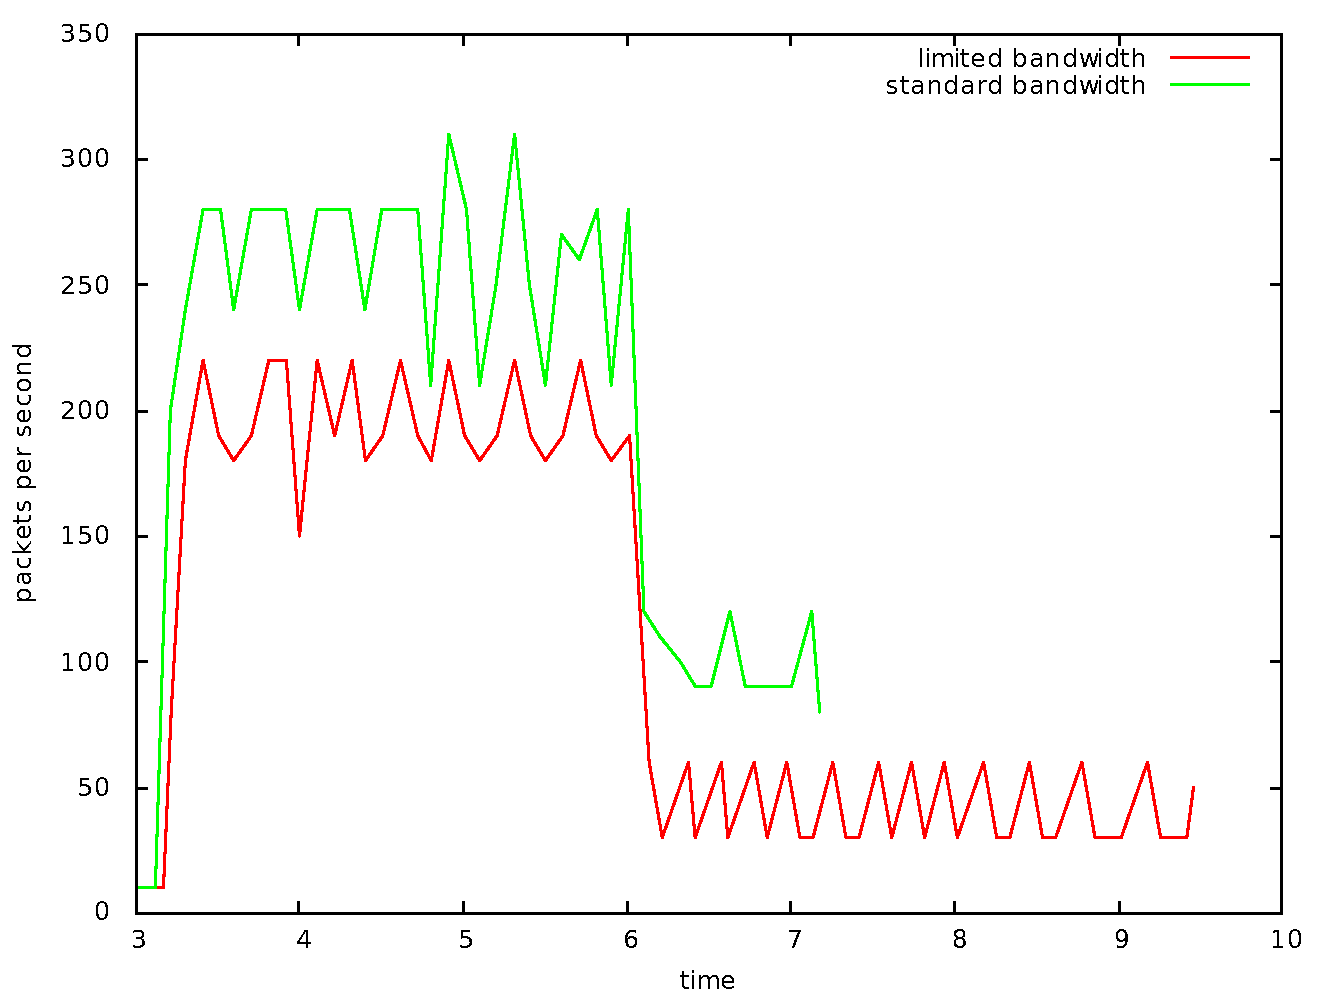
\includegraphics[width=\textwidth]{../part1/q4/plots/4-up.pdf}
    \caption{Upload throughput}
    \label{fig:up_limited}
\end{figure}

\subsection{Question 5}

When we impose a fixed bitrate on the CBR connection, we ensure that
this connection never takes more than its preallocated share of
bandwidth. Thus, when we allocate a small percentage of the total
connection bandwidth, we ensure that other connections on the same
link will not suffer from greatly limited performance, since TCP will
not allocate more bandwidth than this fixed rate. TCP can then
dynamically allocate bandwidth to other connections.

% observations from simulation %

We set up a simulation in NS/2 and verified our assertion. We observed
no packet loss, and only a very slight drop in throughput for the
download connection in the period from 3.0s to 6.0s. The speed drop is
due to packets from two different origins arriving at a router and
being inserted into its buffer. Of course, in this scenario, packets
cannot be immediately forwarded to their destination, causing a drop
in throughput, which is small because of the limited amount of packets
being sent by the CBR application.

To improve download performance, we could for example use TCP Reno,
which lowers the congestion window size less drastically when packet
loss occurs. This way, we keep congestion control but do not throttle
the throughput as quickly as we do with TCP Tahoe.

\subsection{Question 6}

\subsubsection{Question 6-1}
A naive response would be to say that we expect performance to stay
the same, since we have ten times the bandwidth for ten times the
users. In actuality, this is not true. Consider the output of a
simulation we made for this scenario.

We can clearly see that all transfers have very variable levels of
throughput when executed simultaneously. The reason for this is that
much more packets are being sent to the router simultaneously; the
router can only process as much packets at a time as fit in its
buffer, so once its buffer is full and more packets arrive, packet
loss will occur. This is expressed in the valleys in the graph
measuring the throughput.

If we have a smaller amount of nodes emitting packets, the probability
of this scenario is also smaller. So, if we have five nodes, packet
loss is less likely to occur than with ten nodes, and this will ensure
a better throughput.

\subsubsection{Question 6-2}

If the same activities are performed at random times, performance will
generally be better than if all activities are performed all at the same
time. The reason for this is that any given point in time, there will
be less than ten users performing the same activity simultaneously (at
least, the probability of this scenario is overwhelmingly greater than
the converse case) and thus less users sharing the same link
bandwidth. On the other hand, if an activity (or multiple activities)
starts while another activity is being performed, TCP will start
throttling all activities. This will cause performance to be hindered
at this point for the other activities.


\section{Exercise 2}
\subsection{Question 1}

In figure \ref{fig:burst_traffic} we have plotted the throughput for
both the long-standing FTP connection and the burst FTP
connections. We observe the following:

\begin{enumerate}
\item We can clearly see sharp drops in throughput for the
  long-standing FTP connection at the 5.0, 10.0 and 15.0 second marks,
  when the FTP bursts begin. This follows from TCP Tahoe's congestion
  control algorithm: the additional burst traffic causes the bandwidth
  to be exceeded, resulting in packet loss. The TCP congestion control
  algorithm will then reduce the congestion window size to a minimum
  and build up again. Still, both connections must share the
  same bandwidth, so the throughput after one of the requests is
  acknowledged will be slower. This is repeated forty times in a span
  of two seconds, resulting in forty throttlings of the transfer speed.
\item The burst traffic throughput reaches a maximum at the end of the
  burst, while the long-standing traffic throughput starts increasing at this
  point and return to a maximum just before the next burst starts. The
  sizes of the files requested by HTTP is not too large, so most
  transfers will be done by this point. Accordingly, the throughput of
  the long-standing connection will slowly increase again, until the
  next burst arrives, packet loss occurs, and the cycle begins anew.
\item Note that he last burst causes a remarkably long drop in
  throughput in the long-standing FTP connection. We believe that this
  is due to the file sizes generated for the last FTP burst, which we
  believe are larger on average than for the other two bursts (as we
  saw in the FTP request logs).
\end{enumerate}

\begin{figure}[p]
    \centering
    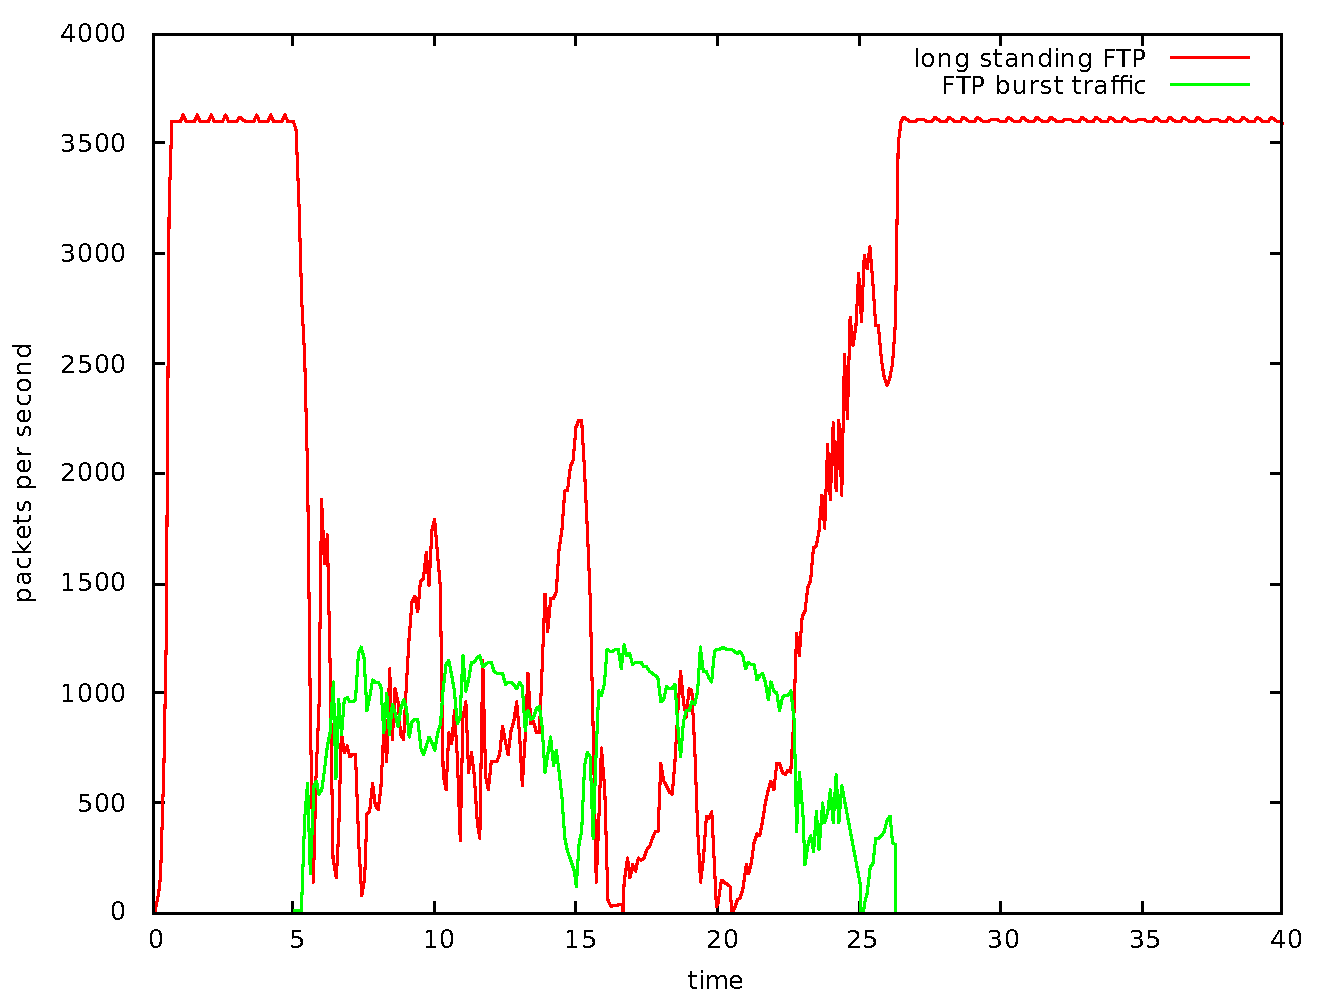
\includegraphics[width=\textwidth]{../part2/q1/plots/1.pdf}
    \caption{Throughput}
    \label{fig:burst_traffic}
\end{figure}


\subsection{Questions 2 and 3}

We can distinguish very clearly the three alternating phases of the
algorithm in figure \ref {fig:aimd}:

\begin{enumerate}
\item the multiplicative increase phase: this phase is entered at the
start of the algorithm or after a multiplicative decrease phase. On
the graph, we can see this as a exponential increase in the congestion
window size from the start value. This is because the number of
packets transmitted during a single transmission round is doubled
after every transmission round.
\item the additive increase phase: this phase is entered once the
congestion window size has reached the current threshold. From this
point on, the window size is increased more slowly until packet loss
occurs. On the graph, we can see a smooth increase in window size
until \ldots
\item the multiplicative decrease phase: starts when packet loss
occurs. The congestion window is set to its start value (in this case,
1) and a new threshold is set, which is half of the previous maximum
congestion window size (except for the first drop, where half of the
initial threshold is chosen). On the graph, we can identify this as a
very sharp drop in window size and a sudden lowering of the threshold.
\end{enumerate}

Let us look more closely at the sawtooth pattern starting a little
before the 12s mark and ending around the 20s mark. We can see that at
the start of the pattern, the congestion window size has a value of
1. The multiplicative increase phase of the algorithm starts at this
point. For a little while, the congestion window size increases until
the threshold is reached around 12s. At this point, we can see the
window size increase slow down, as is reflected by the smooth linear
increase in the graph (congestion window increases by one every RTT);
this is the additive increase phase. This continues until packet loss
occurs around the 15.5s mark. At this point, the multiplicative
decrease phase starts, in which congestion avoidance is active; the
congestion window size drops sharply to its start value, which is
clearly visible on the graph. Once this value is reached, a new
`sawtooth' pattern starts.

\begin{figure}[p]
    \centering
    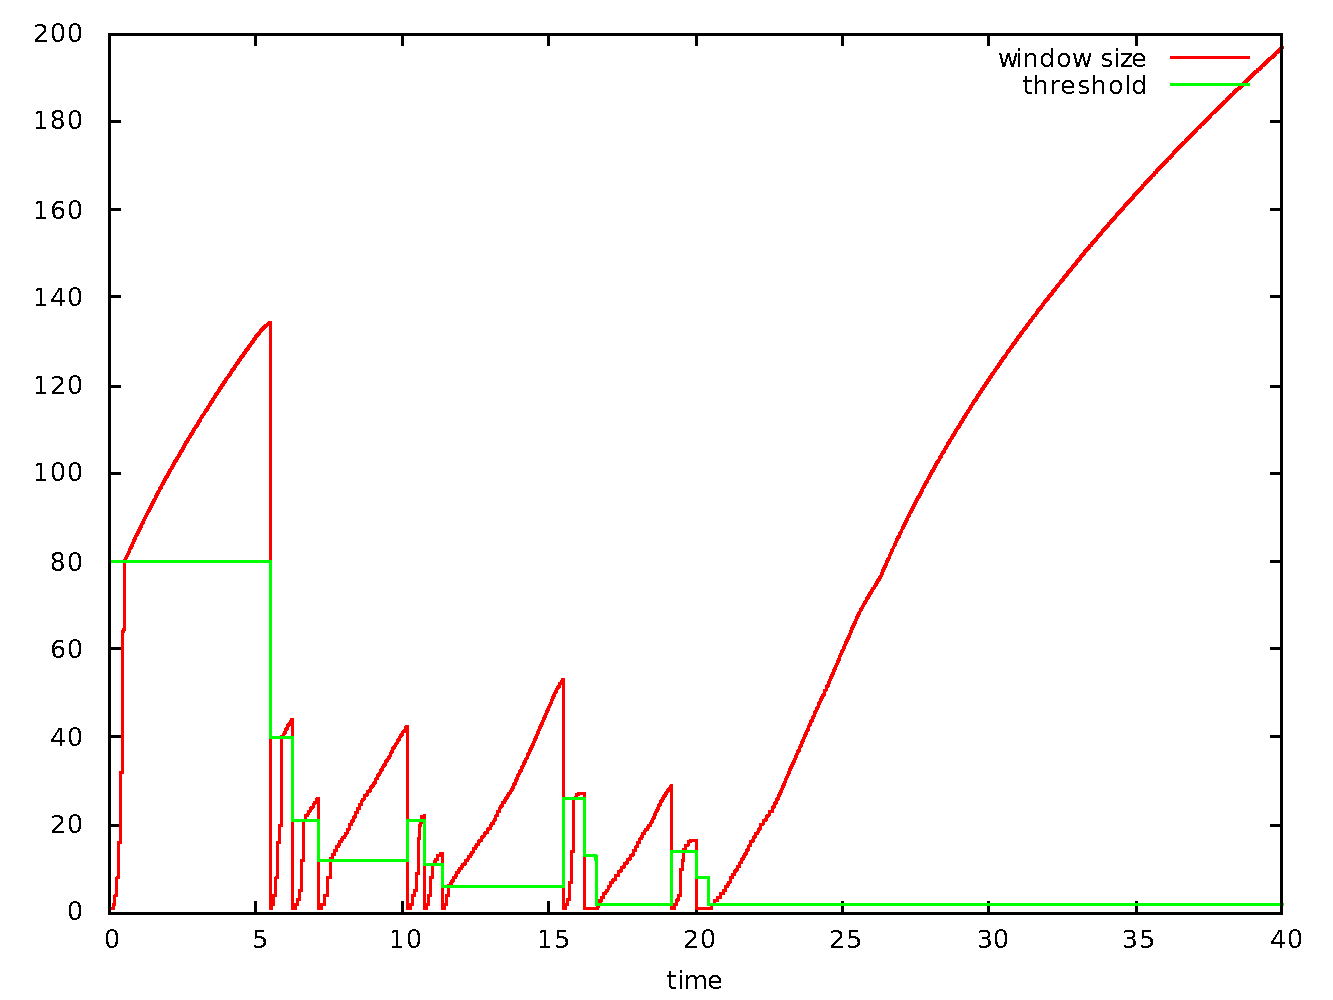
\includegraphics[width=\textwidth]{../part2/q2/plots/algorithm.pdf}
    \caption{Congestion window size and slow start thresholds}
    \label{fig:aimd}
\end{figure}



\subsection{Question 4}

We can see the evolution of the congestion window size and threshold
in figure \ref{fig:aimd_reno}. The figure largely resembles figure
\ref{fig:aimd} except for the fact that the congestion window size is
reset in two different ways: either it is reset to 0 or 1 when a packet
times out, as in Tahoe, or it is reset to a newly calculated size
when packet loss occurs. This size is half of the congestion window
size when the loss occurred; once the congestion window is resized,
the threshold is also set to this value. This is TCP Reno's `fast
recovery'.

For instance, a little after the 15s mark, a timeout occurs and the
congestion window size drops to 1. From here on, it displays the same
behavior as Tahoe until before the 20s mark, when packet loss occurs.
The window size at this point is around 25; accordingly, the next
window size will be 12, and the threshold is also set to this value.

\begin{figure}[p]
    \centering
    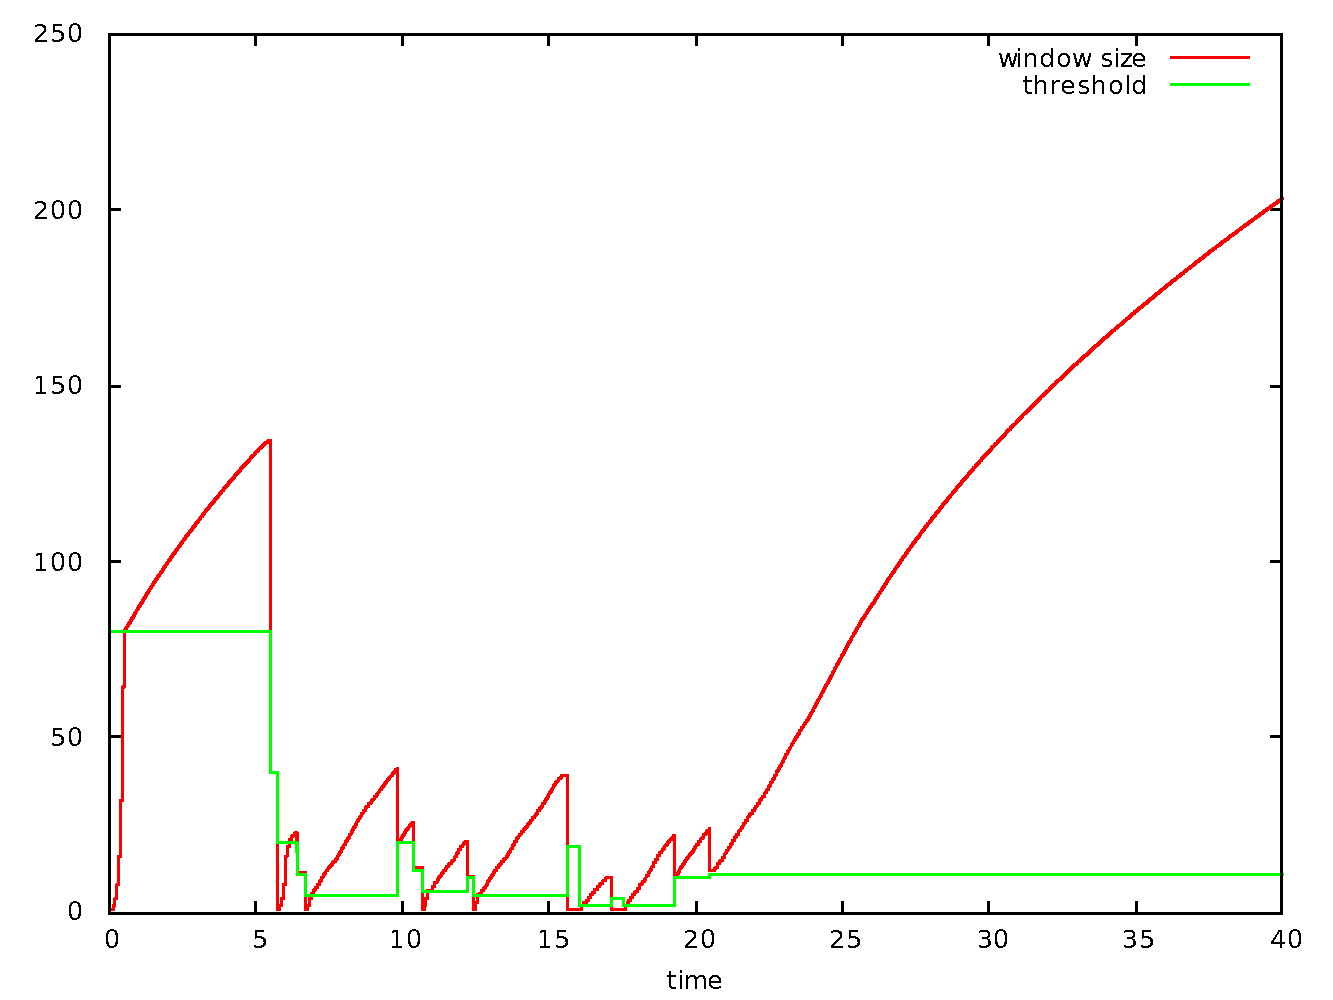
\includegraphics[width=\textwidth]{../part2/q4/plots/algorithm.pdf}
    \caption{Congestion window size and slow start thresholds (with
      the TCP Reno algorithm)}
    \label{fig:aimd_reno}
\end{figure}


\newpage
\section{Source code listings}

\textbf{Warning: we output trace files to stdout; this will mess with
  the terminal display on some systems due to the large amount of data
emitted!}

\subsection{Base setups}
\subsubsection{Exercise 1}
\lstinputlisting[language=Tcl]{/home/xavier/projects/computer_networks_2/practicum/part1/base.tcl}
\subsubsection{Exercise 2}
\lstinputlisting[language=Tcl]{/home/xavier/projects/computer_networks_2/practicum/part2/base.tcl}

\subsection{Exercises}
\subsubsection{Exercise 1.1}
\lstinputlisting[language=Tcl]{/home/xavier/projects/computer_networks_2/practicum/part1/q1/1.tcl}
\subsubsection{Exercise 1.2}
\lstinputlisting[language=Tcl]{/home/xavier/projects/computer_networks_2/practicum/part1/q2/2.tcl}
\subsubsection{Exercise 1.3}
\lstinputlisting[language=Tcl]{/home/xavier/projects/computer_networks_2/practicum/part1/q3/3.tcl}
\subsubsection{Exercise 1.4}
\lstinputlisting[language=Tcl]{/home/xavier/projects/computer_networks_2/practicum/part1/q4/4.tcl}
\subsubsection{Exercise 1.5}
\lstinputlisting[language=Tcl]{/home/xavier/projects/computer_networks_2/practicum/part1/q5/5.tcl}
\subsubsection{Exercise 1.6.1a}
\lstinputlisting[language=Tcl]{/home/xavier/projects/computer_networks_2/practicum/part1/q6/6-1a.tcl}
\subsubsection{Exercise 1.6.1b}
\lstinputlisting[language=Tcl]{/home/xavier/projects/computer_networks_2/practicum/part1/q6/6-1b.tcl}
\subsubsection{Exercise 1.6.2}
\lstinputlisting[language=Tcl]{/home/xavier/projects/computer_networks_2/practicum/part1/q6/6-2.tcl}
\subsubsection{Exercise 2.4}
\lstinputlisting[language=Tcl]{/home/xavier/projects/computer_networks_2/practicum/part2/q4/4.tcl}

\end{document}